\documentclass [11pt,fleqn]{article}

\usepackage{color}
\usepackage{amssymb}
%\usepackage{epsf,psfig,graphicx}
%\usepackage{epstopdf} % TJL ADDED
\usepackage{bm}
\usepackage{epsf,graphicx}
\usepackage{psfrag}
\usepackage{float}
\usepackage{amsmath}
\usepackage[mathscr]{euscript}
\usepackage{color}
\topmargin     -0.60in  % (adjusted for printer bias) 
\headheight      .00in  % (no headers) 
\headsep         .50in  % (top margin + headers + skip) 
\textheight     9.50in  % (instructions: 9 1/8'' min, 9 7/16'' max) 
\textwidth      6.00in  % 2*3.33 + .33 = 6.99 
\oddsidemargin  0.3125in  % (subtracted 1inch bias) 
\evensidemargin 0.3125in 
%\renewcommand{\baselinestretch}{1.5} 
\parindent .0in 
\parskip 10pt 
\usepackage{verbatim}

\newcommand*{\matminus}{%
  \leavevmode
  \hphantom{0}%
  \llap{%
    \settowidth{\dimen0 }{$0$}%
    \resizebox{1.1\dimen0 }{\height}{$-$}%
  }%
}

\font \bigtenrm=cmmi10 scaled\magstep2 
\def \dt {\delta\tau} 
\def \ve {\varepsilon} 
\def \ch {{\cal H}} 
\def \del {\partial} 
\def \be {\begin{equation}} 
\def \ee {\end{equation}} 
\def \beq {\begin{eqnarray}} 
\def \eeq {\end{eqnarray}} 
\def \tv {\tilde v} 
\def \veren {\varepsilon^{\rm ren}_f} 
\def \vef {\varepsilon^0_f} 
\def \su {\uparrow} 
\def \sd {\downarrow} 
\def \CR {\nonumber\\} 
\def \hfb {\hfill\break} 
\def \tb {\bar{t} } 
\def \kb {\bar{k} } 
\def \tbB {\bar{t}_B } 
\renewcommand*{\thefootnote}{\fnsymbol{footnote}}
%\def \ul{#1} {$\underline{#1 }$}
\newcommand{\angstrom}{\textup{\AA}}
\usepackage{authblk}
\usepackage{lineno}
\title{Nanoparticle twinning observed using  correlated x-ray scattering (CXS)}
%\author[1]{ Derek Mendez }
%\author[3]{ Thomas J. Lane}
%\author[1,2]{Jongmin Sung}
%\author[7]{Jonas Sellberg}
%\author[4,6]{Cl\'ement Levard}
%\author[1]{Herschel Watkins}
%\author[7]{Aina E. Cohen}
%\author[7]{Michael Soltis}
%\author[2,5]{Shirley Sutton}
%\author[2]{James Spudich}
%\author[3]{Vijay Pande}
%\author[7]{Daniel Ratner}
%\author[1,7]{Sebastian Doniach} %\thanks{corresponding author: sxdwc@slac.stanford.edu}}

%\affil[1]{Stanford University Department of Applied Physics, Stanford, CA 94305}
%\affil[2]{Stanford University Department of Biochemistry, Stanford, CA 94305}
%\affil[3]{Stanford University Department of Chemistry, Stanford, CA 94305}
%\affil[4]{Stanford University Department of Geological and Environmental Sciences, Stanford, CA 94305}
%\affil[5]{Stanford University School of Medicine, Stanford, CA 94305}
%\affil[6]{Aix-Marseille Universit\'e, CNRS, IRD, CEREGE UM34, 13545 Aix en Provence, France}
%\affil[7]{SLAC National Accelerator Laboratory, Menlo Park, CA 94025}

%\renewcommand\Authands{ and }
\author{Doniach group}
\date{}
\begin{document} 
%\setpagewiselinenumbers
%\linenumbers
\maketitle

\delimitershortfall=-1pt

\begin{center}
\section*{Abstract}
\end{center}
Twinning was observed from 32,000 isotropic solution exposures recorded at the Japanese x-ray free electron laser. These data were collected for a routine detector geometry calibration prior to a separate wide-angle experiment. Each exposure was a snapshot of roughly $90,000$ gold particles (each 60 nanometers across) suspended freely with random orientations. Twinning, which is readily observed using electron microscopy techniques, can go unnoticed in conventional x-ray scattering measurements which require long exposures that average away azimuthal variations (e.g. wide angle x-ray scattering / WAXS ). By using correlated x-ray scattering (CXS) analysis, we resolved a signal indicative of a basic twinning structure common to the nanoparticles. We are able to distinguish the twinning model from another hypothetical model with a precision of [insert precision]. We hope this experiment sheds a new light on CXS as a technique for resolving local structural details from solution measurements.

\section{Introduction}
Correlated x-ray scattering (CXS) is an emerging field which involves recording many snapshot exposures of an ensemble of randomly oriented mono-disperse molecules or particles, and employing photon intensity correlation analysis in order to recover a function dependent only on the average internal structure of the objects in the random ensemble[1]. CXS has potential to reveal the structural properties of proteins without the use of crystallization or single particle imaging. An obvious precursor to the study of soft matter CXS is that of nanoparticles (NPs), due to their typically large scattering cross sections. NP suspensions are used in chemical catalysis, and their chemical properties are directly related to  the overall shape and atomic structure of the NPs themselves [2,3]. As such, there is a need for additional characterization methods. A lot of work has been done describing the thermodynamics and kinetics of NP growth and formation [4,5]. As a result it is known that smaller NPs (tens of nanometers) tend to form complicated twinning structures, e.g. icosahedral twins [6,7,8]. Previously, twinning has been observed using electron microscopy and tomography [9,10], where one images single NP projections. On the other hand, conventional powder x-ray diffraction measurements, used widely in industry to characterize ensembles of NPs, are isotropic averages and don't show signs of twinning (Figure \ref{fig:contrast}). In what follows we will show how CXS combined with the exceptional brightness of the SACLA beam can reveal twinning from many snapshot exposures of a solution of gold NPs.

\begin{figure}[H]
\begin{center}
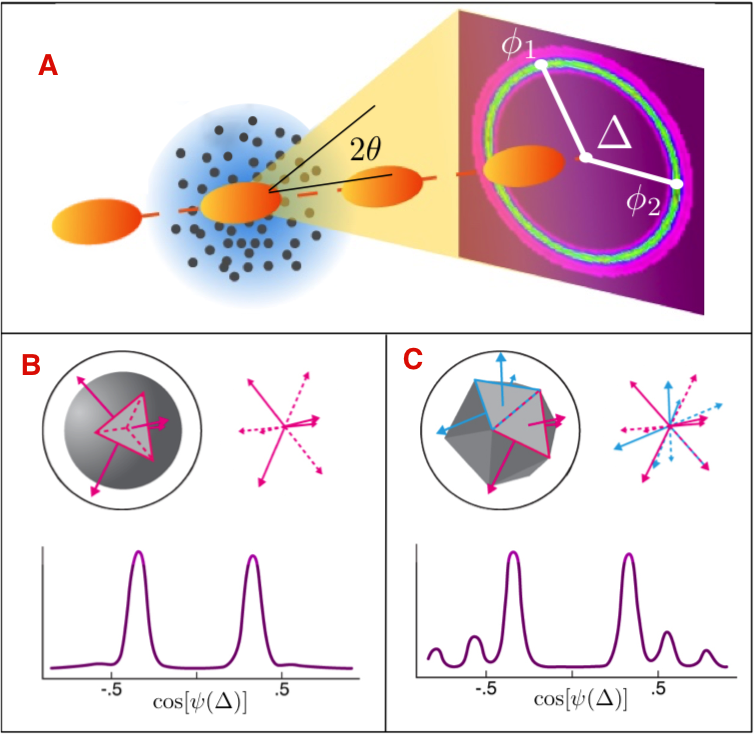
\includegraphics[width=\textwidth,height=\textheight,keepaspectratio]{./fig1_new_version2.png}
\end{center}
\caption{Distinguishing twinned NPs from roughly spherical NPs using CXS. \textbf{A)} A snapshot exposure of a solution of nanoparticles. Whether or not the NPs are twinned is unclear from the powder pattern alone. Highlighted in green is the $\{111\}$ Bragg ring. \textbf{B)} A bulk face-centered-cubic NP with a spherical boundary and the corresponding $\{111\}$ CXS signal. One can imagine these particles form as the $\{111\}$ planes expand in their respective directions (the Bragg vectors). The expanding planes are outlined in pink, showing a regular tetrahedron. The plotted correlation signal has two pronounced peaks at $\pm (1/3)$, corresponding to the $70.5^{\circ}$ and $109.5^{\circ}$ angles between the planes of a regular tetrahedron. This would be the expected $\{111\}$ correlation from any bulk FCC crystal. \textbf{C)} An icosahedral twinned FCC nanoparticle and the corresponding $\{111\}$ CXS signal due to a nearest-neighbor twinned unit (highlighted in blue and pink). The icosahedron is formed by 10 nearest-neighbor twinned units - each unit consisting of two regular FCC tetrahedrons related by a reflection about the common plane (referred to as the twin boundary). As the icosahedron forms, dislocations and other defects serve to stabilize the NP, but here we only plot the CXS which would result from one pair of twins. The CXS signal shows pronounced peaks at $\pm (1/3), \pm (5/9), \pm (7/9)$, which correspond to the angles between between all pairs of $\{111\}$ planes in a nearest-neighbor twin unit. The increased complexity of the CXS signal is paralleled by the cluster of blue and pink Bragg vectors. Artwork courtesy of Gregory M.~Stewart (SLAC).}
\label{fig:contrast}
\end{figure}

\section{Background}
If an x-ray source is bright enough, then an object exposed to it can scatter photons into at least two directions, $\bm q_1$ and $\bm q_2$. While the orientation of this object is random, the angle defined by $\bm q_1$ and $\bm q_2$ 

\be \label{cpsi}
\cos (\psi) = (\bm q_1 \cdot \bm q_2)/(q_1 \, q_2 )
\ee

is not; it is constrained by the object's internal atomic structure. A crystalline NP scatters photons into discrete Bragg vectors $\bm q_{hkl}$. Let a detector define a set of pixels $\{\bm q\}$, where each $\bm q \in \{\bm q\}$ has a unique position in reciprocal space. Let $\omega$ be a triple of Euler angles defining an NP orientation relative to some axis (e.g. that of an x-ray beam). An NP at orientation $\omega$ can scatter photons into the detector provided

\be \label{condition}
\hat{\bm R}_\omega \cdot \bm q_{hkl} \in \{\bm q\}
\ee

where $\hat{\bm R}_\omega$ is an operator which rotates the NP from some pre-defined arbitrary orientation into $\omega$. We assume a small fraction of NPs in solution are oriented such that condition (\ref{condition}) is met for two Bragg vectors, $\bm q_{hkl}$ and $\bm q_{h'k'l'}$. When an NP is oriented as such, and if it scatters photons into both $\bm q_{hkl}$ and $\bm q_{h'k'l'}$, then these photons are said to be correlated. This double Bragg scattering produces angular intensity correlations between pairs of pixels in $\{\bm q\}$ whose angular separation $\psi$ is defined by

\be \label{hklcorr}
\cos(\psi_{hkl,h'k'l'}) =\frac{ \bm q_{hkl} \cdot \bm q_{h'k'l'} } {q_{hkl}\, q_{h'k'l'}} 
\ee

The angle $\psi_{hkl,h'k'l'}$ is also the interplanar angle between crystallographic planes $hkl$ and $h'k'l'$. Typically, the pixels $\{\bm q\}$ are arranged on a planar detector, assumed perpendicular to the forward x-ray beam. With such a setup, it is often convenient to express correlations in terms of the azimuthal angle $\phi$ which spans the detector plane $(0 \le \phi \le 2\pi)$. The azimuthal degree of separation, $\Delta = \phi_1  - \phi_2$, between any 2 pixels on the detector can be expressed in terms of (\ref{cpsi}) via

\be \label{project}
\cos(\psi) = \cos( \Delta )\cos( \theta_1)\cos(\theta_2) + \sin(\theta_1)\sin(\theta_2)
\ee

where $\theta$ is the Bragg scattering angle for photons at wavelength $\lambda$, defined by

\be
\sin (\theta)   = \frac{ \lambda  }{ 4\pi } \, q
\ee

(Figure \ref{fig:contrast} A). Geometrically, $\psi$ has maximum when $\Delta=\pi$, hence

\be \label{psimax}
\cos(\psi_{max}) = - \cos( \theta_1)\cos(\theta_2) + \sin(\theta_1)\sin(\theta_2)
\ee

which sets a bound on the correlation angles that can measured in a given experiment. 

In a typical exposure, most NPs will not scatter into the detector, and the ones that do will not be oriented such that they scatter into multiple detectable directions. Therefore, the average exposure is comprised of a large fraction of randomly scattered photons (owing to the orientation randomness in a solution). As such, the correlation signal-to-noise is much less than unity for a single exposure, which has been shown to scale as the square root of the number of averaged exposures, $N_s$ [12]  (in a simplified theoretical framework where there is no inter-particle interaction or interference terms). We consider an exposure to be a snapshot, meaning the NPs should not be moving significantly throughout the exposure duration. This is accomplished automatically with the femtosecond timescale pulses of the SACLA facility [13].  CXS can also be conducted at synchrotron radiation facilities, provided  that the sample is prepared accordingly, and that it is cooled during exposure [14,15]. 

\section{Theory}
Each gold NP has a well-defined face-centered-cubic (FCC) lattice structure. For simplicity, we will only discuss correlations arising from the $\{111\}$ family of planes. There are 4 distinct $\{111\}$ planes: $111$,$11\bar 1$,$\bar 1 1\bar 1$,$1\bar 1 \bar 1$, and the mirror-symmetric planes, $\bar 1\bar 1\bar 1$,$\bar 1\bar 1 1$,$1 \bar 11$,$\bar 1 1 1$.  Photons scattered from these crystallographic planes from an ensemble of randomly oriented NPs will form a Bragg ring at  $q_{111} = 2\pi / d_{111} $ where $d_{111}$ is the inter-planar spacing. Let 

\be
\bm Q_{111} = \{\bm q_{111}, \bm q_{11\bar 1},\bm q_{\bar 1 1\bar 1},\bm q_{1\bar 1 \bar 1},\bm q_{\bar 1\bar 1\bar 1},\bm q_{\bar 1\bar 1 1},\bm q_{1 \bar 11},\bm q_{\bar 1 1 1}\}
\ee

be the set of $\{111\}$ Bragg vectors. If we let 

\be
F( \bm q_1, \bm q_2) =  (\bm q_1 \cdot \bm q_2)/(q_1 \, q_2 ) = \cos( \psi )
\ee

then we can determine analytically which angles give rise to correlations by defining the sequence

\be \label{psiset}
\bm \Psi_{111} = \{ F( \bm q_1, \bm q_2)\, \big | \, (\bm q_1, \bm q_2 \ne \bm q_1) \in \bm Q_{111}\, ,\,  \arccos [F( \bm q_1, \bm q_2)]  \, \le \,  2\theta_{111}   \}
\ee 

where we made use of (\ref{psimax}). Note, $F(\bm q, -\bm q) = -1$ corresponding to a correlation angle of $\pi$ is not included in the sequence as this angle is not measurable using conventional flat detectors. Rigorously,

\be
\bm \Psi_{111} = \{ -x_1, -x_2, ... -x_{12}, x_1, x_2, ... x_{12} \}
\ee 

where $x_i = 1/3\,\,\, (1 \le i \le 12 )$, provided that $ 2\theta_{111} \, \ge \, \arccos \left[(-1/3)\right ]$ for the experiment (Figure \ref{fig:contrast} B). 

Keep in mind that this analysis assumes that each gold NP is a single FCC domain. It is well known that smaller FCC NPs are not single crystal domains. Instead, they tend to form complicated twinning structures composed of many tetrahedral sub-units [ref]. The reciprocal space of these structures is more complex than that of a single domain NP, but this complexity is hidden in standard powder diffraction images; the twins all scatter into the same Bragg rings. CXS, however, is sensitive to twinned NPs. Consider the following simple model for two FCC tetrahedrons joined by a twinning plane. Let each face of the tetrahedrons be a $\{111\}$ plane. When joined, the tetrahedrons will have 1 plane in common, referred to as the twinning plane. The twins atomic coordinates are related to one another by a reflection about this plane. We refer to this twinned structure as a nearest-neighbor twin (NNT). Larger structures, e.g. decahedrons and icosahedrons, can be assembled with NNTs (Figure \ref{fig:contrast}c). We call the twins "twin$_A$" and "twin$_B$".  In our model, twin$_A$ is oriented relative to twin$_B$ via a rotation of $\pi$ about its $(111)$ direction. This operation is given by the matrix

\be \label{twinmat}
\mathbf T = \begin{bmatrix}
       \frac{-1}{3} & \frac{2}{3} & \frac{2}{3}           \\[0.3em]
       \frac{2}{3} & \frac{\matminus 1}{3}           & \frac{2}{3} \\[0.3em]
       \frac{2}{3}           & \frac{2}{3} & \frac{-1}{3}
     \end{bmatrix}
\ee

During an exposure, photons can scatter from each twin into separate Bragg vectors and become correlated on a detector which captures them. We refer to these correlations as inter-twin correlations. Let us define the set of Bragg vectors for the NNT model as 

\be
\bm Q^{A,B}_{111}\,\, =\,\, \bm Q_{111} \, \cup \, \{  \mathbf T  \cdot \bm q \, \big |\, \bm q \in \bm Q_{111} \}
\ee

We can now predict where NNTs will give correlations using this new set of vectors: 

\be \label{psisetab}
\bm \Psi^{A,B}_{111} = \{ F( \bm q_1, \bm q_2)\, \big | \, (\bm q_1, \bm q_2 \ne \bm q_1) \in \bm Q^{A,B}_{111}\, ,\,  \arccos [F( \bm q_1, \bm q_2)]  \, \le \,  2\theta_{111}     \}
\ee

For experiments with sufficiently large $2\theta_{111}$, (\ref{psisetab}) will contain only values $\pm (1/3), \pm (5/9), \pm(7/9)$ (Figure \ref{fig:contrast}C). Rigorously, 

\beq
\bm \Psi^{A,B}_{111} &=& \{\, x_1, ... x_{36}, -x_1, ... -x_{36},  \\
&&\,\,\,\, y_1, ... y_{12}, -y_1, ... -y_{12}, \\
&& \,\,\,\, z_1, ... z_6, -z_1, ... -z_6 \, \}
\eeq

where $x_i = 1/3\,\,\, (1 \le i \le 36 )$, $y_i = 5/9\,\,\, (1 \le i \le 12 )$, $z_i = 7/9\,\,\, (1 \le i \le 6 )$.  We assume $  2\theta_{111} \, \ge \, \arccos \left[(-7/9)\right ]  $ during the experiment. We expect that the magnitude of the intensity correlations should agree with the frequency of values in this sequence. This is in line with our simple simulations (Figure \ref{fig:contrast C}), though we did not test this rigorously.

Note we reached these conclusions by considering the atomic structure of a single NP; the information content of CXS depends solely on the scattering factor of the individual particle in solution. For the case of NPs, the scattering factor is a relatively simple function in reciprocal space, however CXS analysis is easily extended to soft matter experiments [ref].

Depending on the growth process, gold NPs have been observed to grow into many complicated twinned shapes, referred to as multiply-twinned particles (MTPs). In an MTP, there are additional correlations which can arise due to next-nearest-neighbor twins and so-forth, but the magnitude of such correlations is diminishing, as there are always more nearest-neighbor twins. 

\section{The Experiment}
Here we will report on the successful measurement of CXS for gold NPs at the SACLA beam facility in Japan. 60 nanometer gold NPs were purchased from Nanopartz Inc. [ref] and suspended in LCP (lipid cubic phase, [ref]) at a concentration of 40 mg/mL. The viscous solution was injected into the beam as a constant stream using a  hamilton 7780 syringe needle with inner diameter 130 $\mu m$. The SACLA beam was focused down to a roughly $1.5 \times 2.4 \mu m ^2$ spot size, and from these numbers we estimate roughly $9 \times 10^4$ 60 nm particles in the beam. 

The beam repetition rate was 30 Hz. The femto-second pulses were measured using an MPCCD 8-panel detector [ref] in a wide-angle setup, with a beam energy of $8.6 keV$ and a maximum scattering angle of $3.4 \, \angstrom^{-1}$. Gain calibrations were provided by SACLA [ref], and dark current measurements (detector readouts with the shutter closed) were roughly performed every $5\times 10^3$ exposures and used to adjust for electronic noise common to CCD detectors. With this setup we acquired $1.6\times 10^5$ snapshot exposures of gold NPs. For the analysis we worked solely with the $\{111\}$ Bragg ring.

The goal of the analysis was to determine the angles $\psi$ which show angular intensity correlations at the $\{111\}$ Bragg ring, and to compare the results with the values in (\ref{psiset}) and (\ref{psisetab}). In this way we hope to elucidate whether the NPs are bulk-FCC or twinned.  

Conventional CXS analysis involves computation of angular correlations in the azimuthal component of the planar detector [ref]

\be \label{cor111}
C_{s,111}(\Delta) = \sum_{i=0} ^{N_\phi-1} \, n_s(q_{111},\phi_i)\, n_s(q_{111}, \phi_i+\Delta)
\ee

Here, $n_s(q,\phi)$ defines the interpolated polar intensity recorded by a pixel at $\bm q$ on the planar detector during snapshot $s$, and $\phi_i = i\,\times (2\pi/N_\phi) $. The correlations are then summed

\be
C_{111}(\Delta) = \sum_{s}^{N_s} C_{s,111}(\Delta)
\ee

and one can use (\ref{project}) to express the resulting signal in terms of $\cos(\psi)$.

\section{Results}

As previously reported [ref], straightforward computation of (\ref{cor111}) is dominated by artificial correlations associated with the experiment. Examples of these correlations include pixel talk, detector shadows, and scattering anisotropies due to an inhomogeneous sample (Fig \ref{fig:raw_dif} a).

Rather then summing each shot, we instead chronologically sort the shots, subtract consecutive exposures who's average mean intensities are within some pre-chosen, non-optimized value, and then correlate the differences. The main assumption is that consecutive exposures have roughly the same artificial asymmetries. Consider a shadow appearing on the detector for a series of exposures; each exposure in the series has the same shadow, therefore subtracting the exposures from one another before correlating the pixels should suppress correlations induced by the shape of the shadow. In this way, the correlations in each exposure are due to the NPs themselves. In reality, the number of photons in each xFEL pule fluctuates wildly, so we must account for this difference as well, which we do by dividing each exposure by it's median intensity. This so-called difference correlation method idea was briefly mentioned in an early reference by Zvi Kam [ref].

With the difference correlation method, we see that our data agree with the predicted CXS signal for gold NNT particles (Figure \ref{fig:raw_dif}b). Without the use of CXS, it would not be possible to tell whether the gold NPs were twinned using x-ray scattering alone. Note that this measured CXS signal represents that of the average gold NP in solution, therefore we do not expect perfect agreement with our simple NNT model. Further, electron microscopy suggests that gold NPs are most likely MTPs, which gives reason that the signal should deviate from that of simple NNT particles, as one would have to include next-nearest neighbor twins etc. in the modeling.

MTPs are commonly observed as decahedrons or icosahedrons. As it turns out, a decahedron cannot be comprised of purely FCC tetrahedrons and still be space-filling [ref]. Early on, a hypothetical model was proposed wherein the FCC lattice within each twinned subunit was strained in order that the decahedron be completely space filling with no dislocations or other defects [ref]. Though it is currently well understood that dislocations and other defects are energetically preferred and stable components of nanoparticle structure, comparing this hypothetical strained model with that of our pure twinning model demonstrates the precision of CXS [Figure].

\section{Conclusion}
Advances in x-ray instrumentation and sources have just now reached a critical point from which CXS has become feasible [ref]. Consequently, the technique itself is in it's infancy. The true power in a CXS measurement is the size of it's parameter space. Here we reported on the measurement of intensity correlations at a single scattering vector, namely $q_{111}$ for gold FCC crystals. In fact, more information is contained in the cross correlations and auto correlations of all the probed scattering angles. As sample injection and data collection tools continue to improve, so should the ability to refine the angular intensity correlation functions hidden within snapshot x-ray measurements.

\begin{figure}[h]
\begin{center}
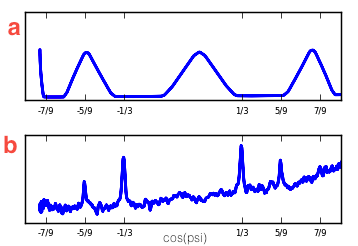
\includegraphics[width=\textwidth,height=\textheight,keepaspectratio]{./raw_dif.png}
\end{center}
\caption{\textbf{a)} Computation of $C_I(\Delta)$ for 174k exposures of gold NP solution. Shows the strong artificial correlation signal associated with experimental noise terms. b) Computation of $\widetilde C_I(\Delta)$ for 87k pairs of exposures. Without further processing, the CXS signal arising from the gold NPs in solution is clear, and clearly shows that the gold NPs are twinned.}
\label{fig:raw_dif}
\end{figure}


\section*{References}

1. Kam Z. 1977 Determination of macromolecular structure in solution by spatial correlation of scattering fluctuations. Macromolecules 10:927–934. (doi:10.1021/ma60059a009)

2. Narayanan R and El-Sayed MA ,2005, Catalysis with Transition Metal Nanoparticles in Colloidal Solution: Nanoparticle Shape Dependence and Stability J. Phys. Chem. B, 109, 12663-12676

3. Radha Narayanan and Mostafa A. El-Sayed, Shape-Dependent Catalytic Activity of Platinum Nanoparticles in Colloidal Solution, Nano Lett., Vol. 4, No. 7, 2004

4. Marks, L. D. Modified Wulff Constructions for Twinned Particles. J. Cryst. Growth 1983, 61, 556‚àí566.

5. Ringe E dx.doi.org/10.1021/jp401566m | J. Phys. Chem. C 2013, 117, 15859‚àí15870

6. Stepwise Evolution of Spherical Seeds into 20-Fold Twinned Icosahedra Mark R. Langille et al. Science 337, 954 (2012); DOI: 10.1126/science.1225653

7. C.Y. YANG Journal of Crystal Growth 47 (1979) 274—282

8. C.Y.YANG, M.J.YACAMAN K.HEINEMANN Journal of Crystal Growth 47 (1979) 283—290

9. Marks, L. D.; Smith, D. J. High-Resolution Studies of Small Particles of Gold and Silver 0.1. Multiply-Twinned Particles. J. Cryst. Growth 1981, 54, 425‚àí432.

10. Chien-Chun Chen et al Nature 496, 74–77 (04 April 2013) doi:10.1038/nature12009

11. Friedel G (1913) Sur les symetries cristallines que peut reveler la diffraction des rayons Rontgen. Comptes Rendus hebdo-madaires de l’Academie des Sciences 157:1533–1536

12. Kirian RA,Schmidt KE,Wang X,Doak RB,Spence JCH. 2011 Signal, noise, and resolution in correlated fluctuations from snapshot small-angle X-ray scattering . Phys. Rev. E 84, 011921. (doi:10.1103/PhysRevE.84.011921)

13. Neutze R,Wouts R,van der Spoel D,Weckert E,Hajdu J. 2000 Potential for biomolecular imaging with femtosecond X-ray pulses. Nature 406, 752–757. (doi:10.1038/35021099)

14. Kam Z,Koch MH,Bordas J. 1981 Fluctuation X-ray scattering from biological particles in frozen solution by using synchrotron radiation. Proc. Natl Acad. Sci. USA 78, 3559–3562. (doi:10.1073/pnas.78.6.3559)

15. Mendez et al, 2014,  Observation of correlated X-ray scattering at atomic resolution, Phil Trans R Soc B 369: 20130315


\end{document}






